\documentclass[10pt,xcolor=dvipsnames,compress]{beamer}

\usepackage{danny_theme}
\usepackage{danny_style}
\usepackage{hyperref}
%\usepackage[algoruled,longend]{algorithm2e}
\usepackage{array}
\usepackage{graphicx}
\usepackage{amsmath}
\newcolumntype{C}{>{\centering\arraybackslash} m{1.3in} }
\newcolumntype{M}{>{\centering\arraybackslash} m{1.in} }
\everymath{\displaystyle}
\long\def\/*#1*/{}

\beamertemplatenavigationsymbolsempty


%===============================================================================
% 					  Presentation Title and Author  
%===============================================================================
\title[Supercapacitor Inadequecy]{
Inadequecy Representation in\\ Models of Supercapacitor Batteries}
%\subtitle{}

\author[Danial Faghihi]{Danial Faghihi}

\institute[ICES]{Institute for Computational Engineering and Sciences (ICES)\\
$\quad~$The University of Texas at Austin
}

\date[Wed May 24, 2017]{PECOS Inadequecy Meeting\\
Wednesday May 24, 2017}
%===============================================================================
%===============================================================================



\begin{document}

%===============================================================================
% SLIDE 00
%===============================================================================
\begin{frame}
\titlepage
\end{frame}

%===============================================================================
% SLIDE 00
%===============================================================================
\begin{frame}
\frametitle{Outline}
\vfill

\vspace{0.7in}
\tableofcontents
\vspace{0.7in}

\vfill
\end{frame}



%%%%%%%--------------------------------------------------------------------------------------------------------------------------
\section{Model Description}
%%%%%%%--------------------------------------------------------------------------------------------------------------------------
%===============================================================================
% SLIDE 00
%===============================================================================
\begin{frame}
\frametitle{Outline}
\vfill

\vspace{0.7in}
\tableofcontents[currentsection,currentsubsection] 
\vspace{0.7in}

\vfill
\end{frame}


%===============================================================================
% SLIDE 03
%===============================================================================
\begin{frame}
\frametitle{Governing Equations}
\vfill

\begin{columns}
\begin{column}{.65\textwidth}
\begin{block}{electrode}
\textbf{Current density} following Ohm's law:
\begin{itemize}
\item Matrix phase :
$
\mathbf{i}_1 = -\sigma\nabla\phi_1
$
\item Solution phase:
$
\mathbf{i}_2 = -\kappa\nabla\phi_2
$
\end{itemize}
$\phi_1$, $\phi_2$: potentials,\\
$\sigma$, $\kappa$: electronic/ionic conductivity.
%

\vspace{0.1in}
\textbf{Conservation of charge:}
\vspace{-0.1in}
\begin{equation*}
-\nabla \cdot \mathbf{i}_1 =  \nabla\cdot \mathbf{i}_2 = a {i}_n
\vspace{-0.1in}
\end{equation*}
$a$: interfacial area per unit volume \\
${i}_n$: current transferred from the matrix to the electrolyte\\
$
{i}_n = \underbrace{C \frac{\partial}{\partial t} \blue{\eta}}_{\rm double-layer} +
\underbrace{{i}_0 ( \exp (\frac{\alpha_aF}{RT} \blue{\eta}) - \exp (-\frac{\alpha_cF}{RT}\blue{\eta})}_{\rm faradaic})
$

\vspace{0.07in}
\begin{center}
overpotential: 
$
\blue{\eta =  \phi_1 - \phi_2}
$
\end{center}

\end{block}
\end{column}
%-----------------------------
\begin{column}{.30\textwidth} 
\begin{center}
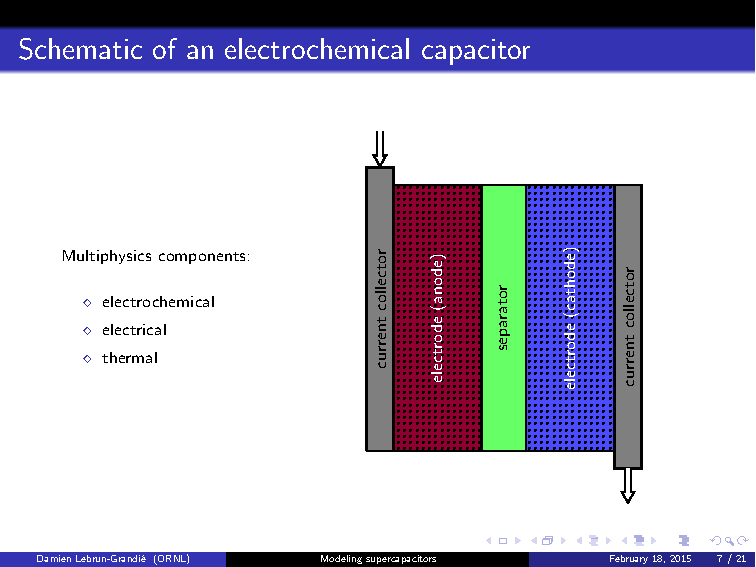
\includegraphics[trim = 2.4in 0.42in 0.7in 0.9in, clip, width=.7\textwidth]{figs/supercap_schematic.pdf}  
\end{center}
\begin{block}{collector}
\begin{equation*}
\mathbf{i}_1 = -\sigma\nabla\phi_1
\end{equation*}
\begin{equation*}
-\nabla \cdot \mathbf{i}_1 = 0
\end{equation*}
\end{block}
%%
\begin{block}{seperator}
\begin{equation*}
\mathbf{i}_2 = -\kappa\nabla\phi_2
\end{equation*}
\begin{equation*}
-\nabla \cdot \mathbf{i}_2 = 0
\end{equation*}
\end{block}
\end{column}
\end{columns}


\vfill
\end{frame}


%===============================================================================
% Slide 04
%===============================================================================
\begin{frame}
\frametitle{High Fidelity Model}
\vfill

\begin{columns}
\begin{column}{.47\textwidth} 
	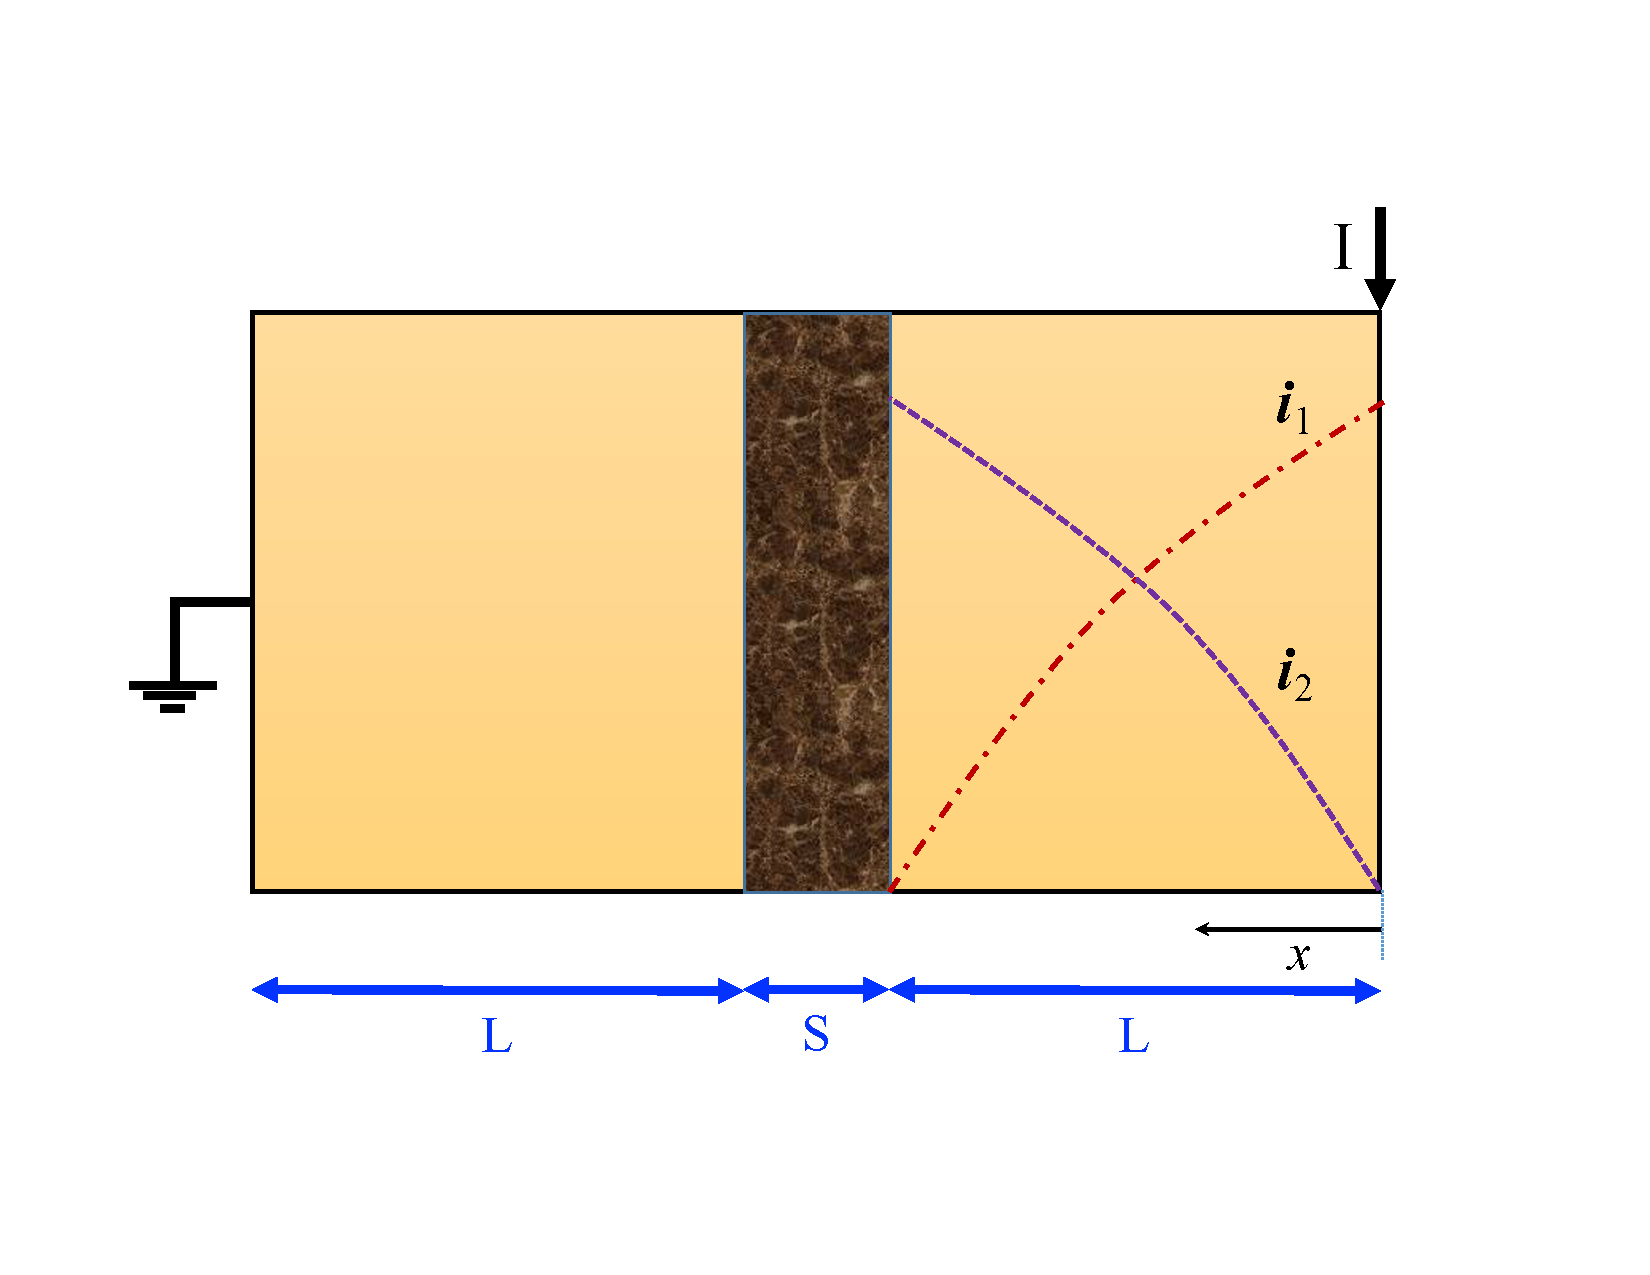
\includegraphics[trim = 0in 1.4in 0in 1.4in, clip, width=1\textwidth]{figs/schematic.pdf}
\end{column}
%-----------------------------
\begin{column}{.47\textwidth}
\begin{itemize}
\begin{small}
\item $\eta(\xi,\tau)$ = overpotential in electrode\\
\item $\gamma = \frac{\kappa}{\sigma}$ : conductivity ratio \\
\item $\xi, \tau$ : dimensionless distance/time \\
\item $I(\tau)$ : dimensionless current
\end{small}
\end{itemize}
\end{column}
\end{columns}
%%====================
\begin{columns}
\begin{column}{.47\textwidth}
\vspace{-0.1in}
\begin{alertblock}{Modeling Assumptions (Sins)}
\begin{enumerate}[i.]

\begin{footnotesize}
\item No Faradaic processes:
current transferred from matrix to the solution phase goes towards only charging the double-layer at the electrode/electrolyte interface.

\item $\phi_1$ is uniformly distributed over the current collector domain (collector is sufficiently thin)
%
%The electrical resistivity of the current collector is low (or it is sufficiently thin) that one can assume uniform distribution of $\phi_1$ over the collector domain: \textit{homogeneous in the $x$-direction}, 

\item There is no electron/ion fluxes cross the top and bottom boundaries
%. Also due to high conductivity of collectors, the voltage over the whole interface on the collector side is negligible (similar to case that tab on the left collector is grounded): \textit{2D domain could be reduced to a quasi-1D domain},

\item The material properties are constant within each layer
\end{footnotesize}

\end{enumerate}
\end{alertblock}
\end{column}
%-----------------------------
\begin{column}{.47\textwidth}
\begin{problock}{High Fidelity (1D) model}
\begin{equation*}\label{eq:HF}
\frac{\partial\eta}{\partial\tau} = \frac{\partial^2\eta}{\partial\xi^2}
\end{equation*}
\begin{equation*}
\left\{\begin{matrix}
\frac{\partial\eta}{\partial\xi}|_{\xi=0} & = & -\frac{\gamma}{1+\gamma}I(\tau)\\
\frac{\partial\eta}{\partial\xi}|_{\xi=1} & = & \frac{1}{1+\gamma}I(\tau) \nonumber\\
\eta|_{\tau=0} 					       & =  & \eta_0(\xi)
\end{matrix}\right.
\end{equation*}
\end{problock}
\end{column}
%-----------------------------

\end{columns}


\vfill
\end{frame}


%===============================================================================
% Slide 05
%===============================================================================
\begin{frame}
\frametitle{Low Fidelity Model}
\vfill


\begin{alertblock}{Modeling Assumptions (Sins)}
\begin{enumerate}[i.]

\item Assuming a quadratically varying profile for overpotential inside the electrodes
\begin{equation*}\label{eq:quadratic}
\eta_{LF} (\xi,\tau)= a(\tau)\xi^2 + b(\tau)\xi + c(\tau)
\end{equation*}
where $a$, $b$, and $c$ can be obtained from PDE+BCs of HF model.

\end{enumerate}
\end{alertblock}

%-----------------------------
\begin{block}{Low Fidelity (0D) model}
\begin{equation*}\label{eq:LF}
\eta_{LF}(\xi,\tau) = 
\frac{1}{2}I(\tau)\xi^2 - I(\tau) \frac{\gamma}{1+\gamma}\xi + {\eta}^{avg}(\tau) - \frac{I(\tau)}{6} + \frac{I(\tau)}{2}\frac{\gamma}{1+\gamma}
\end{equation*}
${\eta}^{avg}$ is the solution of following ODE given appropriate initial condition.

Spatially
averaging the governing equation over the entire domain length
%
\begin{equation*}\label{eq:LF_avg}
\eta^{avg} = \int_0^1 \eta d\xi \qquad \Rightarrow \qquad
\frac{\partial{\eta}^{avg}}{\partial\tau} = I(\tau)
\end{equation*}
\end{block}


\vfill
\end{frame}



%===============================================================================
% Slide 06
%===============================================================================
\begin{frame}
\frametitle{QoI : cell voltage }
\vfill


\begin{alertblock}{Quantity of Interest}
 Potential drop across the system
 \begin{eqnarray*}
 V^{\rm cell}(\tau) &=& \phi_{\rm collector}^L - \phi_{\rm collector}^R \\
 		&=& 2V_0 - 2V^{\rm elect.} - V^{\rm sep.}
 \end{eqnarray*}

where 

$
V^{\rm elect.}(\tau) =  \phi_{\rm 1}|_{\xi=0} - \phi_{\rm 2}|_{\xi=1} = \frac{1+2\gamma}{1+\gamma}\eta|_{\xi=1} - \frac{\gamma}{1+\gamma}\eta|_{\xi=0} 
 - \frac{\gamma}{(1+\gamma)^2}I
$

and

$
V^{\rm sep.}(\tau) =  
I\frac{L_s}{\kappa_s}
$

\end{alertblock}



\vfill
\end{frame}



%%%%%%%--------------------------------------------------------------------------------------------------------------------------
\section{Inadequecy Representation}
%%%%%%%--------------------------------------------------------------------------------------------------------------------------
%===============================================================================
% SLIDE 00
%===============================================================================
\begin{frame}
\frametitle{Outline}
\vfill

\vspace{0.7in}
\tableofcontents[currentsection,currentsubsection] 
\vspace{0.7in}

\vfill
\end{frame}


%===============================================================================
% Slide 07
%===============================================================================
\begin{frame}
\frametitle{Inadequacy Representation}
\vfill


\begin{alertblock}{Objective:}
Based on what we know about the models, develop a representation of inadequacy (\textit{error in QoI}, $\epsilon$) as a parametric model $\mathcal{P}(\boldsymbol{\theta})$ such that 
\begin{equation*}
V^{\rm cell}_{\rm HF} \equiv  V^{\rm cell}_{\rm LF} + \mathcal{P}(\boldsymbol{\theta})
\end{equation*}
\end{alertblock}


\begin{itemize}

\item Parameters of inadequacy model, $\boldsymbol{\theta}$, needs to be calibrated using the data furnished by HF model for simple scenarios, e.g. 

\begin{figure}[h]
    \centering
    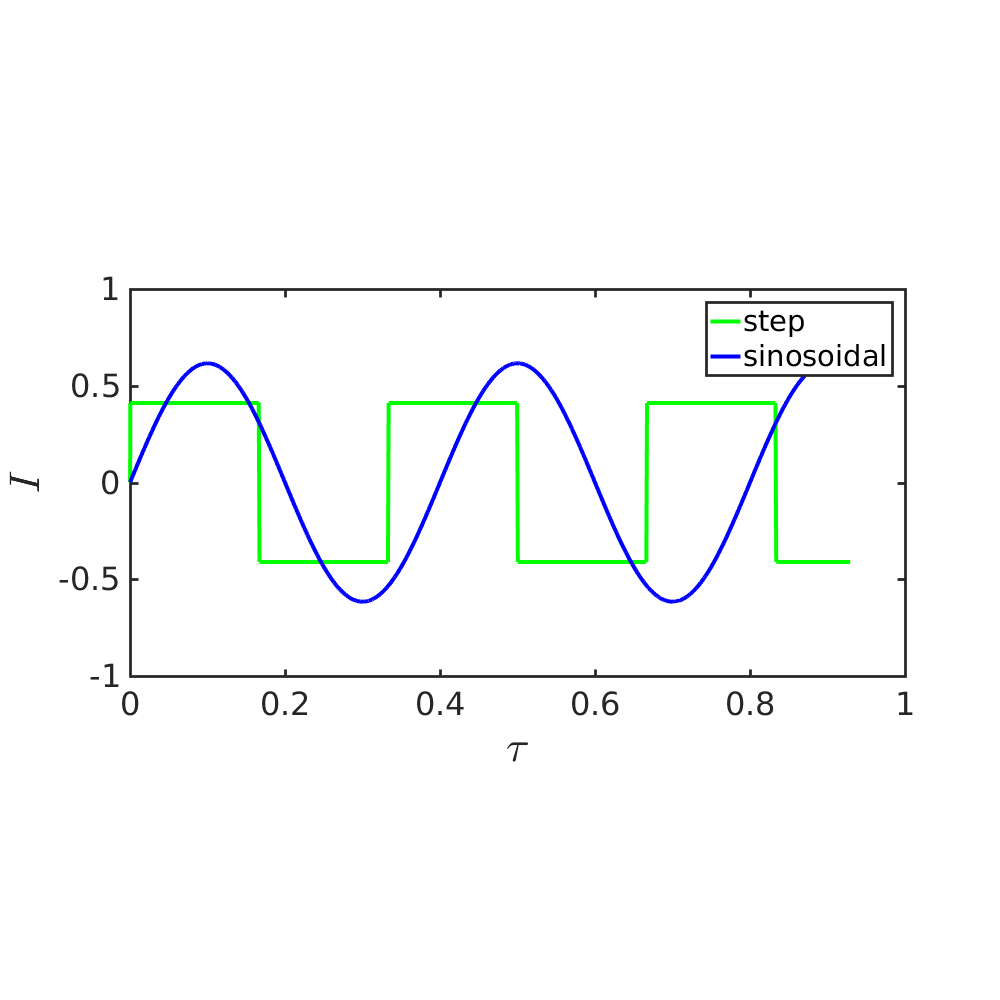
\includegraphics[trim = 0.in 2.4in 0.8in 2.8in, clip, width=0.5\textwidth]{figs/I_scenario.png} 
\end{figure}

\vspace{-0.1in}

\item $\mathcal{P}(\boldsymbol{\theta})$ enables predicting $V^{\rm cell}$ for more complex scenarios outside of the HF data domain along with the associated uncertainty.

\end{itemize}


\vfill
\end{frame}



%===============================================================================
% Slide 07
%===============================================================================
\begin{frame}
\frametitle{Inadequacy Representation}
\vfill


Inadequacy model $\mathcal{P}(\boldsymbol{\theta})$ involves:
\begin{itemize}
\item \textit{Deterministic counterpart:}
Encapsulates our information about the models.

\item \textit{Stochastic counterpart:}
Represents the remaining uncertainty due to lack of information about features of full HF system.
\end{itemize}

\begin{columns}
\column{0.2\textwidth}
\begin{figure}[h]
    \centering
    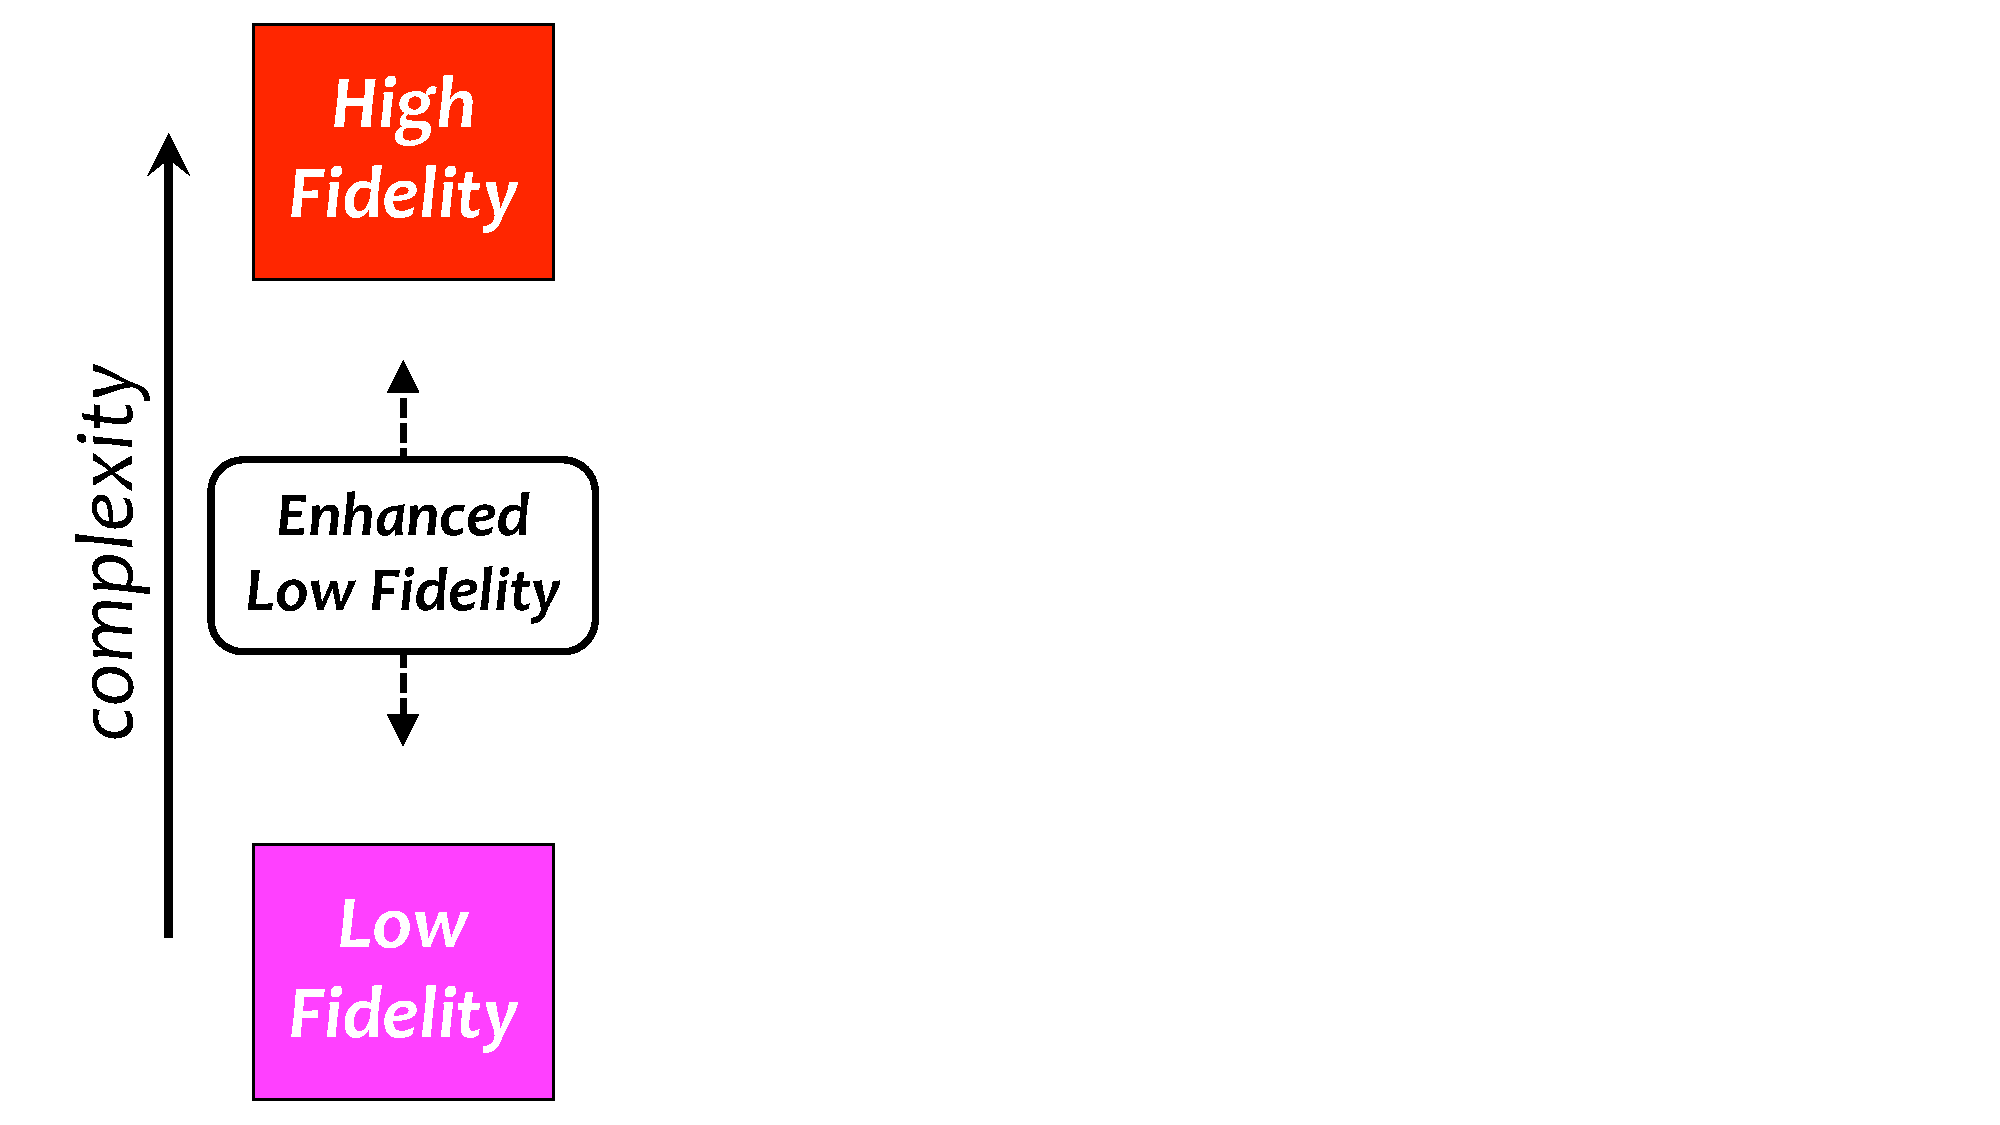
\includegraphics[trim = 0.in 0.in 9.in 0in, clip, width=1\textwidth]{figs/ELFmodel.pdf} 
\end{figure}

\column{0.8\textwidth}

\begin{block}{}

\begin{itemize}
\item The goal is to construct a class of enhanced low fidelity models (intermediate complexities) based on our knowledge about the system, thus,

\begin{itemize}
\item Deterministic part of $\mathcal{P}(\boldsymbol{\theta})$ :
$V^{\rm cell}_{\rm ElF} -  V^{\rm cell}_{\rm LF}$
\item Stochastic part of $\mathcal{P}(\boldsymbol{\theta})$: 
$V^{\rm cell}_{\rm HlF} -  V^{\rm cell}_{\rm ELF}$
\end{itemize}


\item The more complex ELF model:
\begin{itemize}
\item more complex deterministic $\mathcal{P}$ i.e. more parameters
\item more HF data might be required to calibrate 
\item less uncertainty in prediction.
\end{itemize}

\end{itemize}
\end{block}


\end{columns}


\vfill
\end{frame}


%===============================================================================
% Slide 01
%===============================================================================
\begin{frame}
\frametitle{Summary of Models and QoI}
\vfill

\begin{columns}
\begin{column}{.35\textwidth} 
\begin{problock}{HF model}

\begin{equation*}\label{eq:HF}
\frac{\partial\eta}{\partial\tau} = \frac{\partial^2\eta}{\partial\xi^2}
\end{equation*}
\begin{equation*}
\left\{\begin{matrix}
\frac{\partial\eta}{\partial\xi}|_{\xi=0} = & -\frac{\gamma I}{1+\gamma}\\
\frac{\partial\eta}{\partial\xi}|_{\xi=1} = & \frac{I}{1+\gamma} \nonumber\\
\eta|_{\tau=0} 	 =  & \eta_0(\xi)
\end{matrix}\right.
\end{equation*}

\end{problock}
\end{column}
%-----------------------------
\begin{column}{.6\textwidth}
\begin{block}{LF model}
\begin{eqnarray*}
\eta = 
\frac{1}{2}I\xi^2 - \frac{I \gamma}{1+\gamma}\xi +
{\eta}^{avg}(\tau) - \frac{I}{6} + \frac{I\gamma}{2(1+\gamma)}
\end{eqnarray*}
%
\textbf{QoI:}
$
V_{\rm LF}(\tau) = {\eta}^{avg}(\tau) + C_{\rm LF} I(\tau)
$
where
\begin{equation*}
\frac{\partial{\eta}^{avg}}{\partial\tau} = I(\tau)
\end{equation*}
\end{block}

\end{column}
\end{columns}

\vspace{0.5in}

\begin{center}
\textbf{What do we know about HF and LF models?}
\end{center}

\begin{itemize}
\item structure of HF and LF, i.e. ODE, PDE, etc.
\item model respond in a simple (unphysical) case, e.g. constant current. 
\item XXXX


\end{itemize}



\vfill
\end{frame}




\end{document}
